\begin{enumerate}
\item Le nombre de manières de colorier un graphe est le produit des nombres de façons de colorier chaque arc.
\begin{itemize}
\item Si le graphe $G$ est complet, on arua $k$ couleurs possibles pour le premier sommet, $(k-1)$ pour le deuxième, etc\ldots (Le graphe G étant complet, la couleur du premier sommet est nécessairement exclu des autres sommets)

Le $n$\^{ième} sommet pourra être colorié de $k-(n-1)$ manières. D'où :
\[ P_{K_n}(k)=\prod_{i=1}^{n} \left( k-(k-1) \right)\]
ou
\[ P_{Kn}(k)=\prod_{i=0}^{n-1}(k-i) \]
(au choix)

\item Si $G$ est vide, la coloration d'un sommet ne contraint pas la coloration des autres sommet. On obtient :
\[ P_{\overline{K_n}}(k)=k^n \]
\end{itemize}
\item $\chi(G)$ étant, par définition, le nombre minimum de couleurs nécessaires pour colorier $G$, si $k < \chi(G)$ alors le graphe $G$ ne peut pas être colorié par $k$ couleurs. Si $k \geq \chi(G)$ alors il doit y avoir au moins une manière de colorier $G$, celui utilisant $\chi(G)$ couleurs.

On a donc :
\begin{displaymath}
	P_G(k) \left\{ \begin{array}{ll}
	=0 & \textrm{si $k < \chi(G)$} \\
	\geq 1 & \textrm{sinon}
	\end{array} \right.
\end{displaymath}

\item 
\item
\item Utilisons la formule de récurrence trouvée au point précédent, et admettons que pour $P_n$ une chaîne de taille $n$ on a :
\[ P_n(k) = k(k-1)^{n-1} \]

Prenons $A$ le graphe initial :
\begin{eqnarray*}
P_A(k) & = & P_B(k) - P_C(k) \\
&=& \big(P_D(k)-P_E(k)\big)-\big(P_F(k)-P_{P_3}(k)\big)\\
&=& \Big[\big(P_{P_5}(k)-P_{P_4}(k)\big)-\big(P_{P_4}(k)-P_{P_3}(k)\big)\Big]-\Big[\big(P_{P_4}(k)-P_{K_3}(k)\big)-P_{P_3}(k)\Big]\\
&=& P_{P_5}(k)+2P_{P_3}(k)-P_{K_3}(k)+3P_{P_4}(k)\\
&=& k(k-1)^4 +2k(k-1)^2+k(k-1)(k-2)-3(k-1)^3 \\
&=& k(k-1)\big[(k-1)^3+z(k-1)+(k-z)-3(k-1)^2\big]\\
&=& (k^2-k)\Big[(k-1)^2\big((k-1)-3\big)+3k -4 \Big]\\
&=& (k^2-k)[k^3-6k^2+12k-8]\\
&=& k^5-7k^4+18k^3-20k^3+8k
\end{eqnarray*}
Où :

$A$ : \raisebox{-0.5\height}{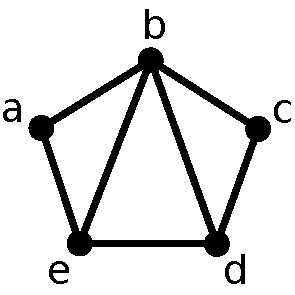
\includegraphics[width=2cm]{files/gAex1.pdf}}

\begin{tabular}{llcll}
$B = A-(e,d) $ : & \raisebox{-0.5\height}{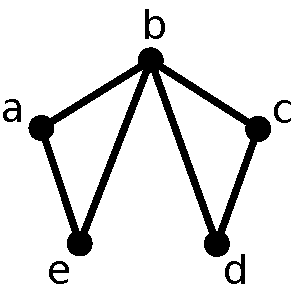
\includegraphics[width=2cm]{files/gBex1.pdf}} & et & $C = A\backslash(e,d)$ : & \raisebox{-0.5\height}{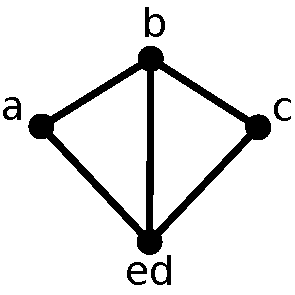
\includegraphics[width=2cm]{files/gCex1.pdf}} \\
$D = C-(a,b)$ : & \raisebox{-0.5\height}{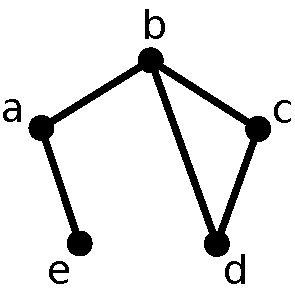
\includegraphics[width=2cm]{files/gDex1.pdf}} & et & $E = C\backslash(e,b)$ : & \raisebox{-0.5\height}{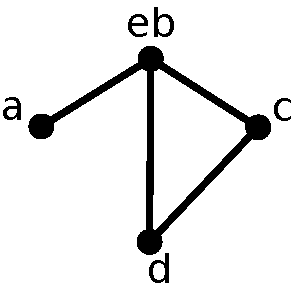
\includegraphics[width=2cm]{files/gEex1.pdf}} \\
$F = C-(b,ed)$ : & \raisebox{-0.5\height}{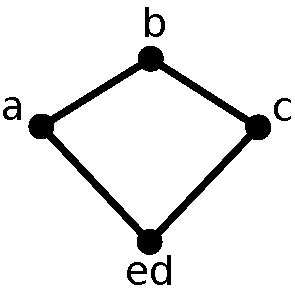
\includegraphics[width=2cm]{files/gFex1.pdf}}& et & $C \backslash(b,ed)P_3$ : & \raisebox{-0.5\height}{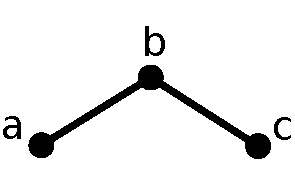
\includegraphics[width=2cm]{files/gC-ex1.pdf}}
\end{tabular}
\end{enumerate}